% !TEX root = ./main.tex
\section{Supplementary Files}
\label{sec:SI_files}
\begin{itemize}
    \item Plasmid Sequences with annotations + RiboJ::YFP
    \item pHelper sequence
    \item Primers
    \item list of restriction sites used in cloning
    \item Gene list
    \item Sequencing Data
    \item List of ordered sequences
\end{itemize}

\clearpage

\section*{Supplementary Figures}
\begin{figure}[H]
    \centering
    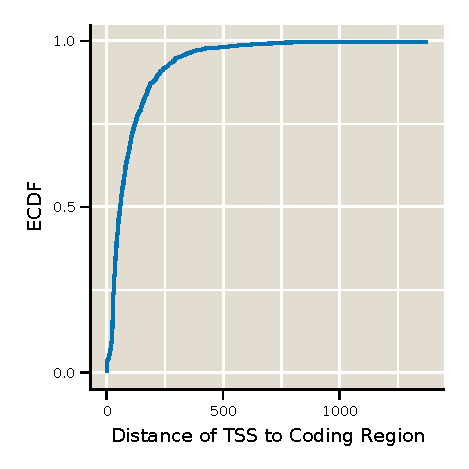
\includegraphics{../figures/tss_CR_distance.pdf}
    \caption{ECDF of distances of transcription start sites to the coding region for every operon in \textit{E. coli} that has a transcription start site annotated in EcoCyc. }
    \label{fig:tss_distance}
\end{figure}


\begin{figure}[H]
    \centering
    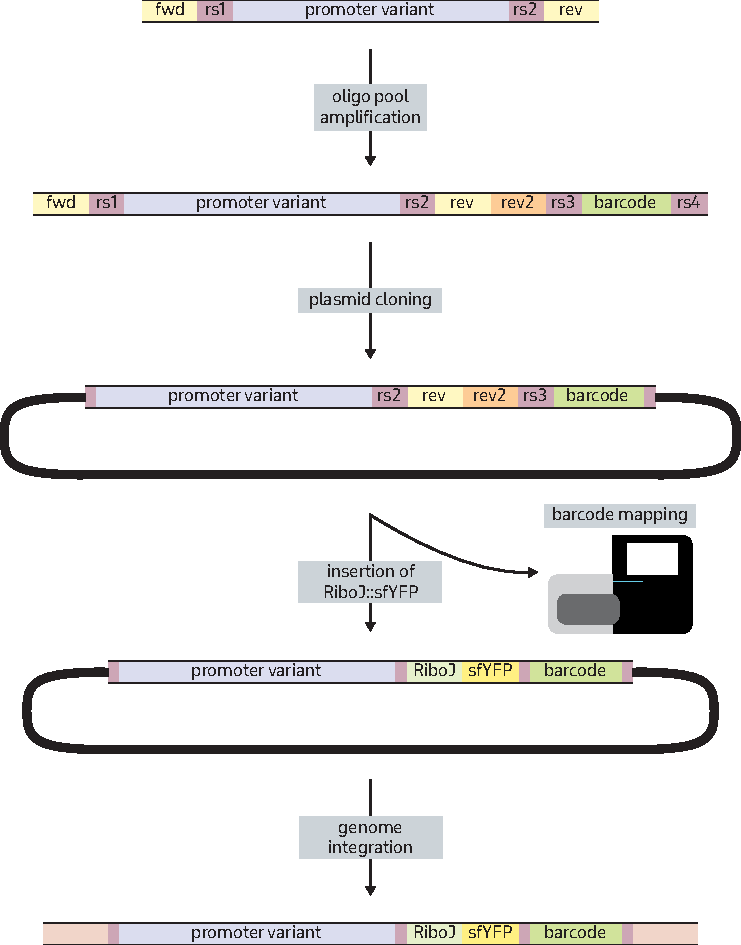
\includegraphics{../figures/cloning_scheme.pdf}
    \caption{Placeholder figure for cloning scheme.}
    \label{fig:cloning}
\end{figure}

\begin{figure}[H]
    \centering
    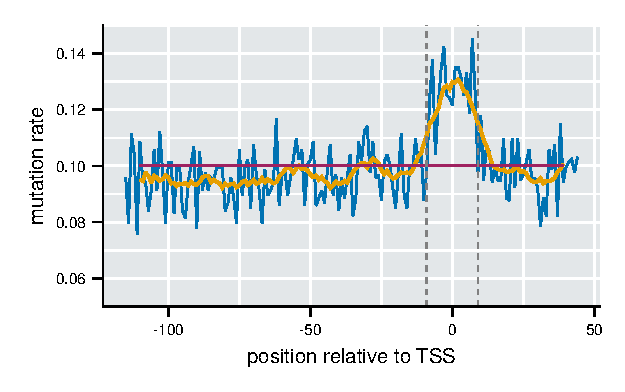
\includegraphics[scale=1]{../figures/dicCp_mutation_rate_oligos.pdf}
    \caption{Mutation rate profile for the promoter of \textit{dicC}. Mutation rate per position (blue) with rolling average over 11 positions (orange) compared to expected average mutation rate of 0.1 (purple). Predicted repressor binding site indicated by grey vertical lines.}
    \label{fig:dicCp}
\end{figure}


\begin{figure}
    \centering
    \includegraphics[scale=1]{../figures/unique_bc_prom.pdf}
    \caption{Number of unique mutated variants for each promoter after barcode mapping. Bars colored in purple indicate that a promoter was duplicated, i.e., there was a second promoter annotated to the same TSS in EcoCyc, for which 1500 variants were created as well, effectively doubling the number of mutated variants for the same promoter. Shown are promoter variants that could be mapped to at least 5 different barcodes.}
    \label{fig:num_uniq_prom_var}
  \end{figure}